\documentclass[10 pt]{article}
\usepackage{graphicx}
\pagestyle{plain}
\usepackage[OT4]{polski}
\usepackage[utf8]{inputenc}
\title{Sprawozdzanie 1\\ \emph{ \textbf{Sortowanie}}}
\author{Paweł Żurek 200404}
\date{10.03.2014}
\begin{document}
\tableofcontents
\maketitle
\section{Wstep}
\textbf{Do posortowania zbioru losowo wygenerowanych elementów użyłem : }
\begin{itemize}
\item Qucik Sort ( Sortowanie Szybkie )
\item Merge Sort ( Sortowanie przez scalanie )
\item Heap Sort ( Sortowanie przez kopcowanie)
\end{itemize}
\section{Wyniki}

\paragraph{Wynik dzialania programu\\}
\begin{center}
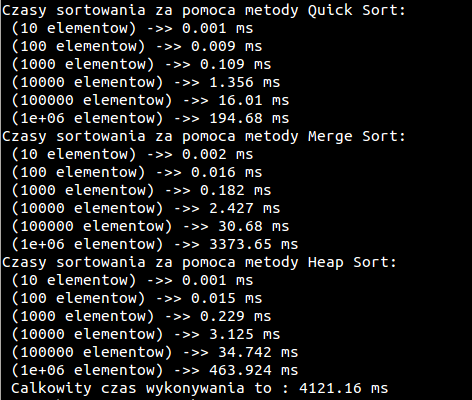
\includegraphics[scale=0.6]{WYKONANIE.png}
\end{center}

\paragraph{Dane wyświetlone za pomoca wykresu ( wykres dostępny osobno w pliku wykres.pdf) \\}
\begin{center}
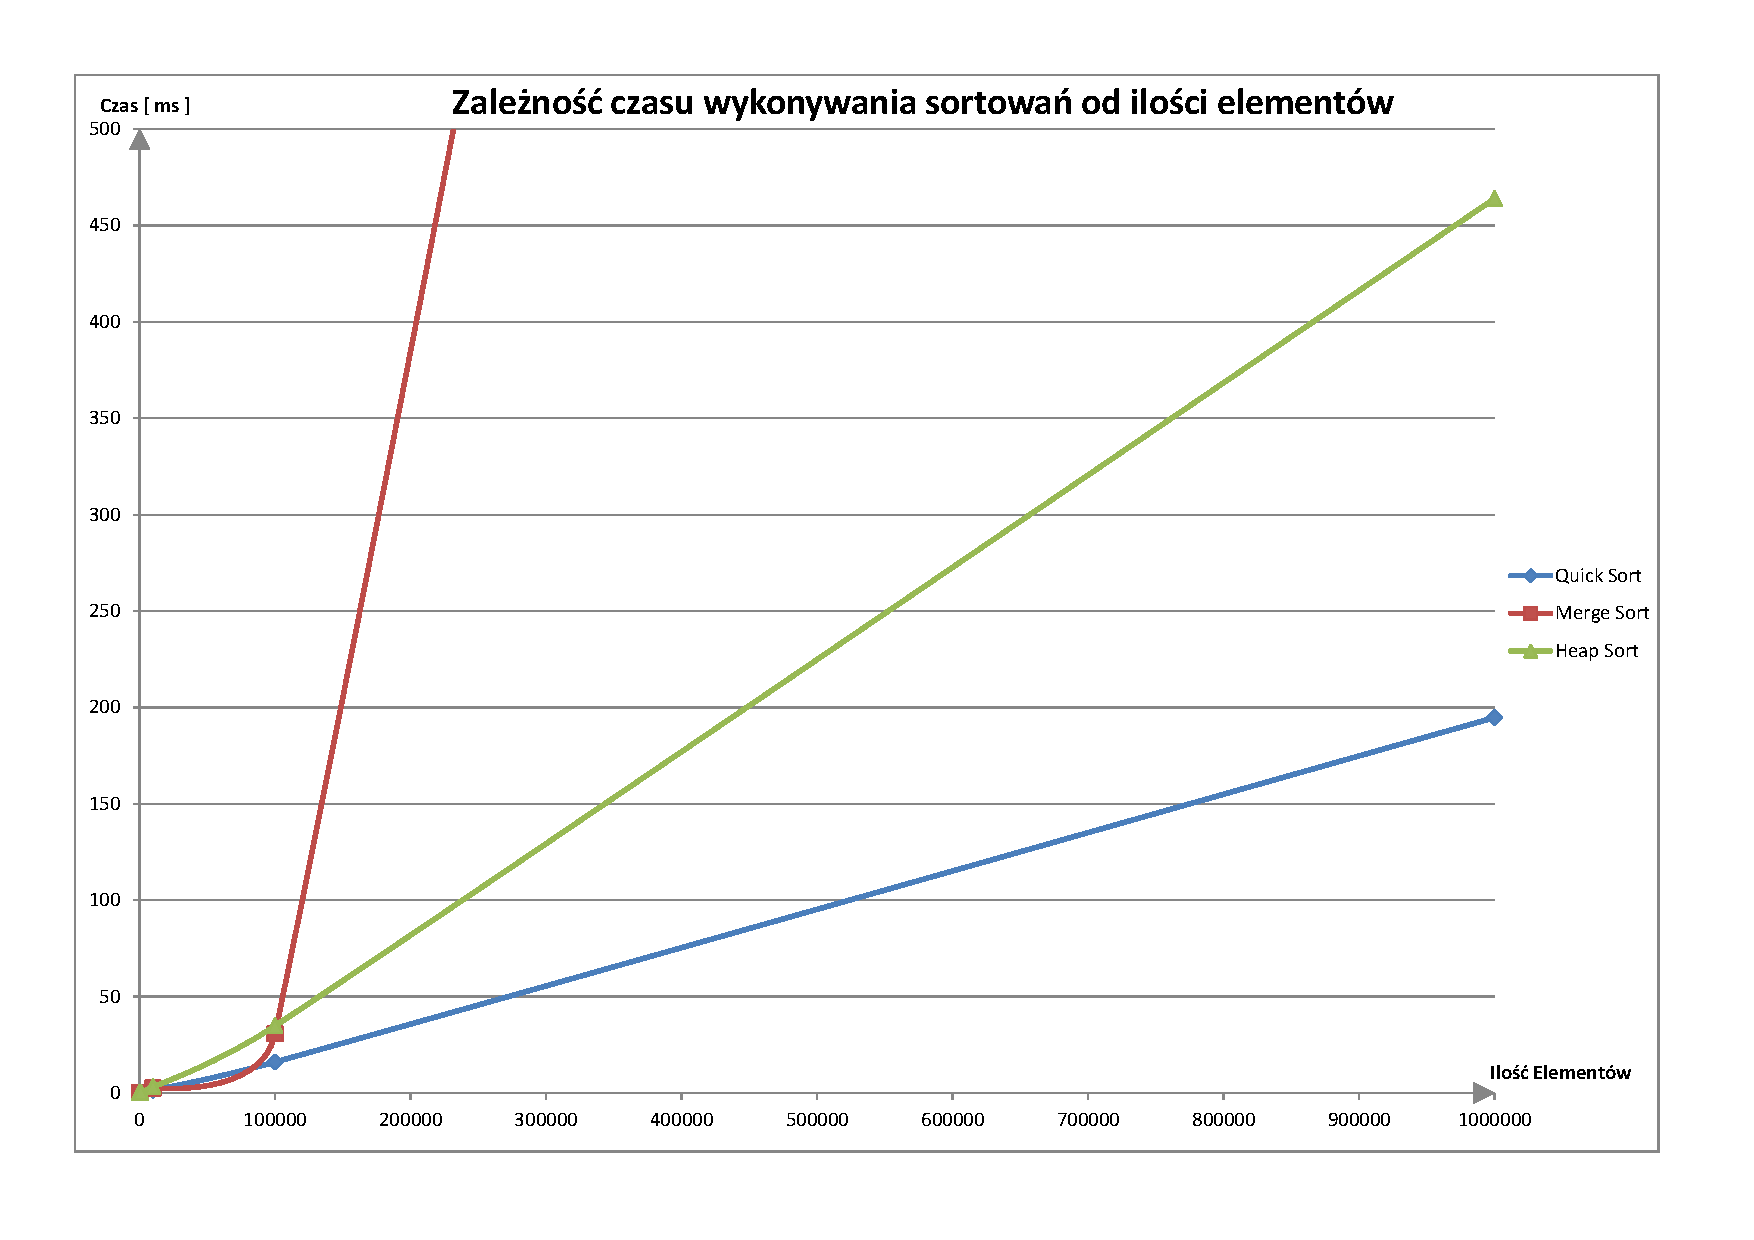
\includegraphics[scale=0.4]{wykres.pdf}
\end{center}
\section{Wnioski:}
\begin{itemize}
\item Algorytm Quick Sort okazał się najszybszy. Prawdopodobnie jest to spowodowane prostotą tego algortymu (
opiera się na Buble Sort, co jest chyba najprostszym algorytmem możliwym ). W przeciwieństwie do
sortowania bąbelkowego, Quick Sort dzieli za każdym razem problem na dwie części, co znacznie przyśpiesza
proces.
\item Algorytm Merge Sort zdecydowanie najwolniejszy. Jest to prawdopodobnie spowodowane tym, że jako
jedyny spośród tych trzech, podczas jego wykonywania jest tworzona dynamicznie tablica pomocnicza.
Wydaje mi się, że to znacznie spowalnia tę metodę.
\item Mimo tego, iż Heap Sort jest dosłownie trochę wolnijszy od Quick Sort, zawsze będę wybierał ten drugi
algorytm ( o ile będzie to możliwe ) ze względu na jego prostotę.

\end{itemize}

Dokumentacja program dostępna w pliku pdf o nazwie ''Dokumentacja'' ( zapisana w \LaTeX u) oraz w doxygen ie ( dostępna w
pliku : dox/html/index.html )

\end{document}